% !TeX spellcheck = en_US
\addscenariosection{1}{Clash Scenario}{Blood for Ore}{\images/mines.png}

\begin{multicols*}{2}

\textbf{Author:} LAAMAKALA

\textit{There is no honor — only victory or death. The weak will fall, the strong will fight, and only one will rule.}

\subsection*{\MakeUppercase{Scenario Length}}
This Scenario plays out over 8-10 Rounds.

\subsection*{\MakeUppercase{Player Setup}}
\textbf{Player Count:} 4

\textbf{Starting Resources:} 16 \svg{gold}, 2 \svg{building_materials}, 1 \svg{valuables}

\textbf{Starting Income:} 15 \svg{gold}, 2 \svg{building_materials}, 1 \svg{valuables}

\textbf{Starting Units:}
\begin{itemize}
  \item A Pack of chosen \bronze\ Units
\end{itemize}

\textbf{Town Buildings:}
\begin{itemize}
  \item \bronze\ Dwelling
\end{itemize}

\subsection*{\MakeUppercase{Map Setup}}
Take the following Map Tiles and arrange them as shown in the Scenario map layout:

\begin{itemize}
  \item 4 × Starting (I) Map Tiles
  \item 8 × Far (II-III) Map Tiles
  \item 5 × Near (IV-V) Map Tiles
\end{itemize}

\subsection*{\MakeUppercase{Victory Condition}}
When a player captures their \nth{6} mine or settlement, all players -- including that player -- take one final turn. After those turns, or at the end of Round 10 (whichever comes first), the game ends. The player controlling the most mines and/or settlements wins. In case of a tie, the tied player with most \svg{gold} wins.

\subsection*{\MakeUppercase{Timed Events}}
\textbf{\nth{2} Round:}
\begin{itemize}
  \item Each Player may Empower one Statistic Card from their Hand.
\end{itemize}
\textbf{\nth{3}, \nth{5} and \nth{7} Round:}
\begin{itemize}
  \item Remove all Black Cubes from the Map except from Learning Stones.
\end{itemize}
\subsection*{\MakeUppercase{Additional Rules}}
\begin{itemize}
  \item A Secondary Hero starting their turn on I or II-III Map Tile gains +1 \svgeven{movement}.
  \item \textbf{Obelisk:} Choose one adjacent Visitable Field and gain its reward. \textit{Visitable once per Faction.}
  \item \textbf{Sanctuary:} Choose 1 \svg{spellpower} from your M&M Deck and add it to your hand, then reshuffle your Deck. \textit{Visitable once per Faction.}
\end{itemize}

\begin{center}
  \vfill
  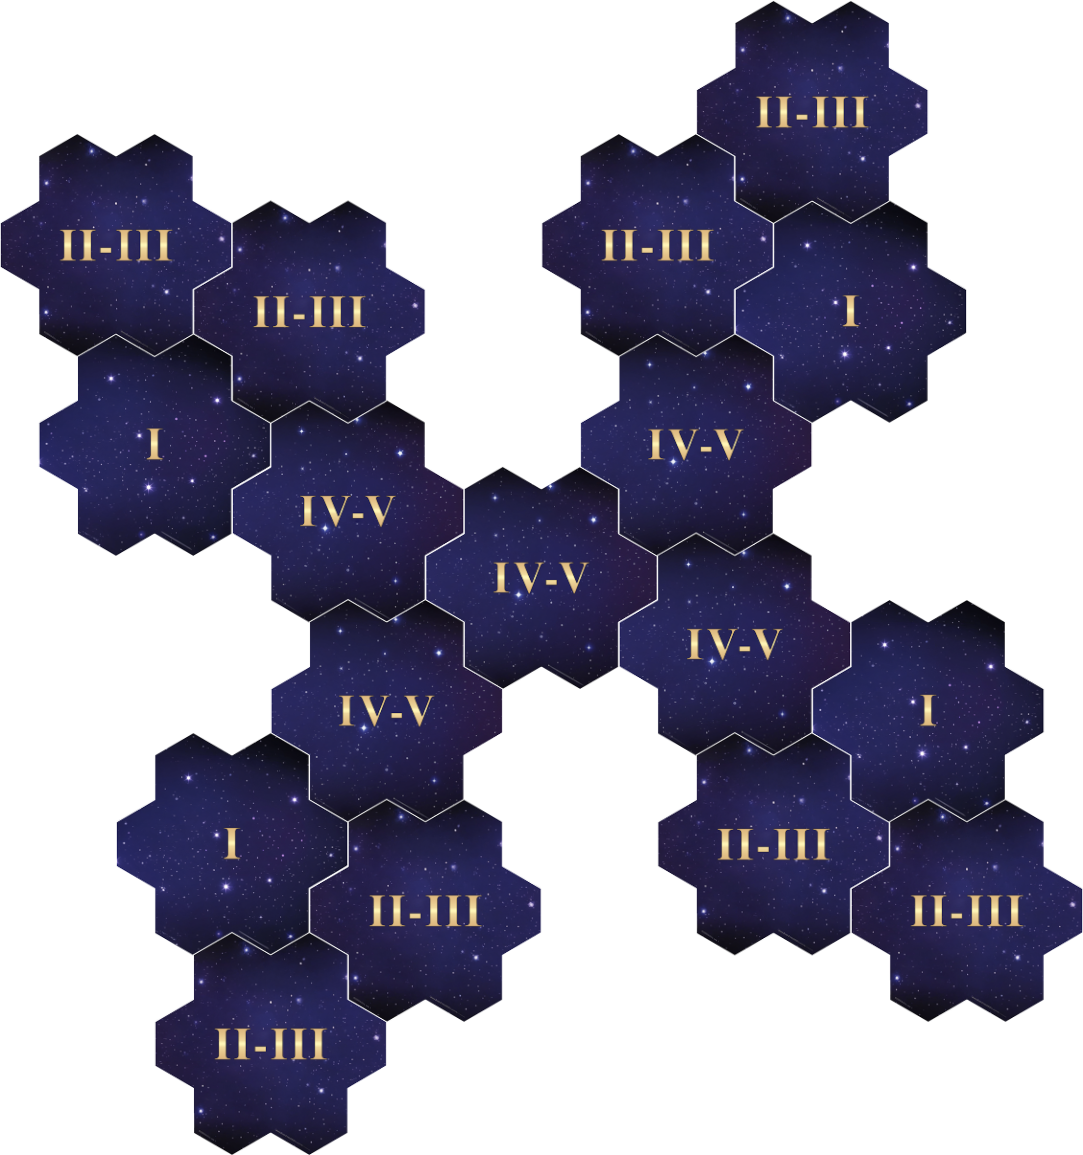
\includegraphics[width=0.93\linewidth]{\maps/blood_ore.png}
  \captionof{figure}{\textbf{SCENARIO MAP LAYOUT}}
  \vfill
\end{center}

\end{multicols*}
